\subsection{Mapping the Crossover and Searching for the QCD Critical Point}
\label{Sec:CP}


%
%%%%%%%%%%%%%%%%%%% Figure PD2 %%%%%%%%%%%%%%%%%%%%%%%%%%%%%%%%%%%%
%\begin{figure}[h!]
%\begin{center}
%\begin{minipage}{0.5\textwidth}
%\hspace*{-12mm}
%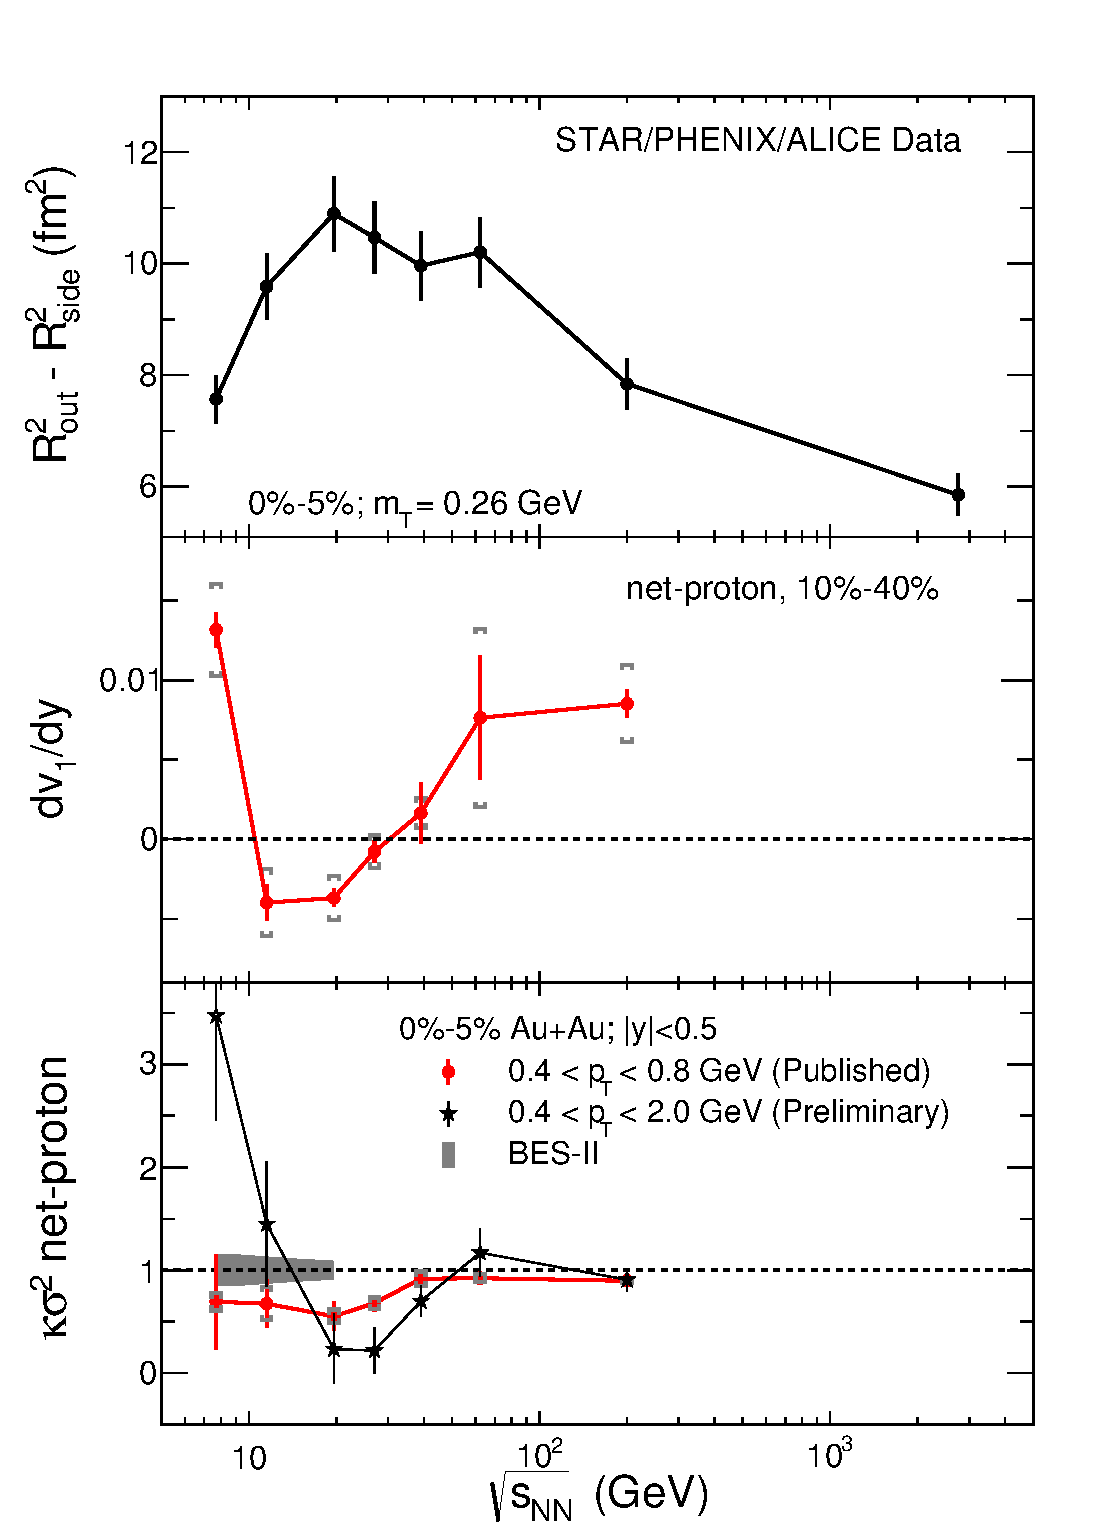
\includegraphics[width=1.22\textwidth]{./fig/bes_compilation_prl_cpod.png}
%\end{minipage}
%\hspace*{2mm}
%\begin{minipage}{0.47\textwidth}
\begin{figure}[!thp]
\vspace{-0.3in}
\begin{center}
\centerline{  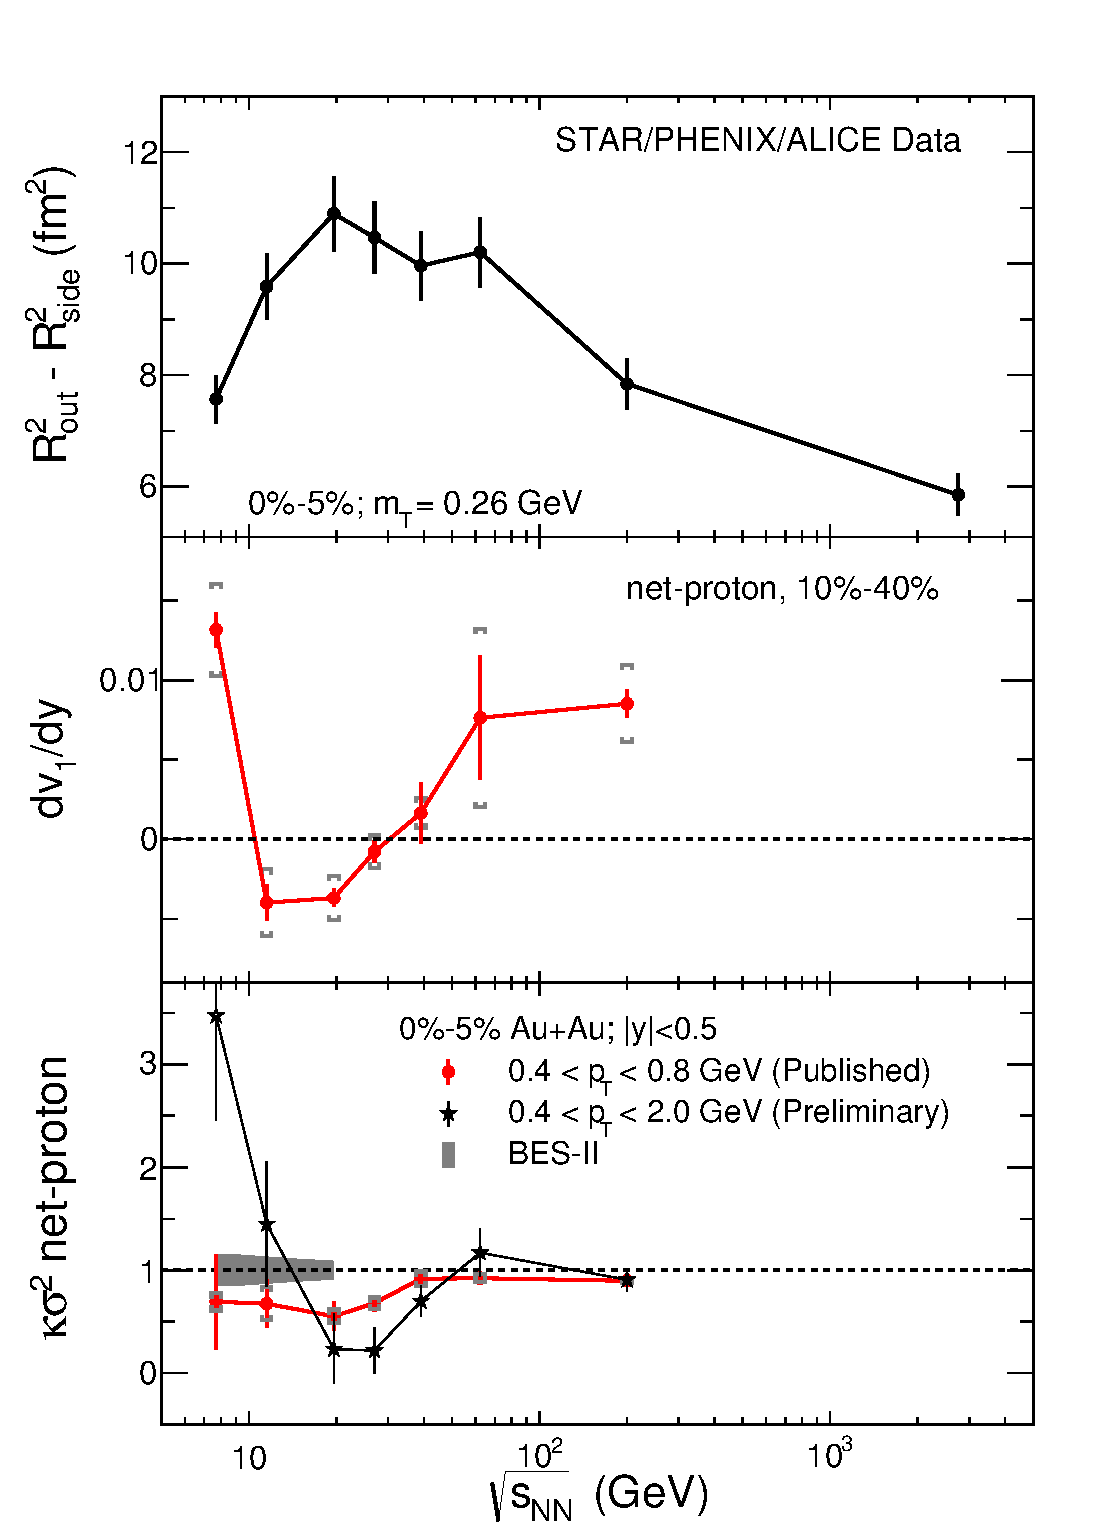
\includegraphics[width=0.7\textwidth]{fig/bes_compilation_prl_cpod.pdf}}
\caption[Observables showing non-monotonic behavior as a function of $\sqrt{s_\mathrm{NN}}$]{Three selected observables
  that all show interesting non-monotonic behavior as functions of collision energy around  $\sqrt{s_\mathrm{NN}}{\,\sim\,}15{-}40$\,GeV.  
    {\bf Top panel:}
  The difference 
  $R_{out}^{2}-R_{side}^{2}$
  between the squared radii
  in the outward and sidewards directions
  measured via two-pion interferometry
  vs. $\sqrt{s_{NN}}$ using STAR~\cite{Adamczyk:2014mxp}, PHENIX~\cite{Adare:2014qvs}, and 
  ALICE~\cite{Aamodt:2011mr}
  data. $R_{out}^{2}-R_{side}^{2}$, 
  reflects the lifetime of the
  collision fireball and was predicted~\cite{Rischke:1996em} to reach
  a maximum for collisions in which a hydrodynamic fluid forms at
  temperatures where the equation of state is softest.  
  {\bf Middle panel:} The rapidity-slope of the net proton directed flow $v_1$,
  $dv_1/dy$. This quantity is sensitive to early pressure gradients in
  the medium.  
  {\bf Bottom panel:} The kurtosis of the event-by-event
  distribution of the net proton (i.e. proton minus antiproton) number
  per unit of rapidity, normalized such that Poisson fluctuations give
  a value of $1$. In central collisions, published results in a
  limited kinematic range~\cite{Adamczyk:2013dal} show a drop below
  the Poisson baseline around $\sqrt{s_{NN}}=$27 and 19.6 GeV. New
  preliminary data over a larger $p_T$ range~\cite{CPODKurtosis},
  although at present still with substantial error bars, hint that the
  normalized kurtosis may, in fact, rise above 1 at lower
  $\sqrt{s_{NN}}$, as expected from critical fluctuations~\cite{Stephanov:2011pb}. 
  The grey band shows the much reduced
  uncertainties anticipated from BES-II in 2018-2019, for the 0-5\%
  most central collisions.}
\label{F-PD2}
%\vspace*{-5mm}
%}
%\end{minipage}
\vspace{-0.1in}
\end{center}
\end{figure}
%%%%%%%%%%%%%%%%%%%%%%%%%%%%%%%%%%%%%%%%%%%%%%%%%%%%%%%%%%%%%%
%



%%%%%%%%%%%%%%%%%%%%%%%%%%%%%%%%%
{\bf The need for BES-II and accompanying advances in theory}
%%%%%%%%%%%%%%%%%%%%%%%%%%%%%%%%%


Several observables from the
first phase of the RHIC Beam Energy Scan program (BES-I, introduced
in Section~\ref{Sec:BES})
exhibit interesting 
non-monotonic behavior as a function of collision energy,
and hence as a function of baryon number chemical potential $\mu_B$.
A selection of such measurements is shown in Figure~\ref{F-PD2}.  
At present, we await with considerable interest
the results from the final run in
the BES-I program at $\sqrt{s_{NN}}=14.5$\,GeV, where the data were taken only
a few months ago, since for a number of important observables the
measurements made previously at and below $\sqrt{s_{NN}}=19.6$\,GeV 
have quite
limited statistics. Nevertheless, it is already possible to see trends
and features in the data that provide compelling motivation 
for both a strong and concerted theoretical response aimed at quantitative
precision as well as for experimental measurements with much higher statistical precision at 
and below $\sqrt{s_{NN}}=19.6$\,GeV 
(i.e. at the largest achievable values of $\mu_B$)
that will be provided by the second phase of the Beam Energy Scan
program (BES-II) in 2018 and 2019. The goal of BES-II, as described
in more detail below, is to follow through in order to turn currently observed trends and
features into definitive scientific conclusions. As discussed in Section~\ref{Sec:RHICUpgrades}, 
the accelerator physicists at RHIC are planning a machine upgrade to
provide electron cooling to increase the beam luminosity at these
energies by about a factor of 10 \cite{BESII}. Targeted new detector
capabilities will also increase the sensitivity to the signals
described below in the BES-II campaign \cite{BESII}.

Experimental discovery of a first-order phase transition or a critical
point on the QCD phase diagram would be a landmark achievement. The
first goals of the BES program, however, have focused on obtaining a quantitative 
understanding of the properties of matter in the crossover region of the 
phase diagram as it changes with increasing $\mu_B$. Available tools
developed over the last few years now make a quantitative comparison
between theory and experiment tractable in the $\mu_B$-range
below any QCD critical point. Success in this effort, in and of itself, would
establish another major and lasting impact of the RHIC program. Questions
that can be addressed in this regime include quantitative study of the
onset of various signatures associated with the presence of
quark-gluon plasma and of the onset of chiral symmetry restoration as
one traverses the crossover region. Data now in hand from BES-I
provide key inputs and impetus toward this goal. Here we give four
examples, intended to be illustrative, of areas where a coherent
experimental and theoretical effort is expected to have substantial
impact on our understanding of QCD. In each case we note the
substantial impact expected from the additional measurements
anticipated during the BES-II:

{\bf 1.} The directed flow observable $dv_1/dy$ for net protons has been 
found to feature a dip as a function of collision energy (see middle panel 
in Figure~\ref{F-PD2}), with a minimum at energies somewhere between 
$\sqrt{s_{NN}}=11.5$ and 19.6\,GeV \cite{Adamczyk:2014ipa}. This has 
long been predicted in qualitative terms as a consequence of the 
softening of the equation of state in the transition region of the phase 
diagram \cite{Brachmann:1999mp,Stoecker:2004qu}. Several theoretical 
groups around the world have now begun hydrodynamic calculations with 
nonzero baryon density, deploying all the sophistication that has been
developed very recently in the analysis of higher energy collisions,
including initial fluctuations and a hadronic afterburner, in
applications to these lower energy collisions. These
hydrodynamic+hadronic cascade calculations will be used to compare the
$dv_1/dy$ data with equations of state in the crossover region of the
phase diagram obtained from lattice calculations via Taylor expansion
in $\mu_B/T$ \cite{Huovinen:2014woa}. This is a program where a
quantitative comparison, successful or not, will be of great interest,
since failure to describe the data could signal the presence of a
first-order phase transition. The precision of a comparison like this
will be substantially improved in 2018-19 when BES-II data will allow
$dv_1/dy$ to be measured for the first time with tightly specified
centrality; the statistics available in the BES-I data sets limit
present measurements to averages over collisions with widely varying
impact parameters \cite{Adamczyk:2014ipa}.

{\bf 2.} A second goal of the hydrodynamic calculations referred to
above will be to use identified particle BES-I $v_2$ data to map, in
quantitative terms, where and how hydrodynamics starts to break down
at lower collision energies, and where, to an increasing extent, $v_2$
develops during the hadron gas phase when viscosities are not small,
{\it i.e.}~where the contribution of the partonic phase to observed measures
of collectivity decreases in importance. A key future experimental
input to this program is the measurement of the elliptic flow $v_2$ of
the $\phi$-meson, which will be obtained with substantially greater
precision in the BES-II program. The first measurements of $v_2$ of
$\Omega$ baryons at these collision energies, also anticipated in
BES-II, will represent a further, substantial advance. Seeing $\phi$
mesons flowing like lighter mesons and $\Omega$ baryons flowing like
lighter baryons in collisions at a given energy would indicate that
the dominant contribution to the collective flow in those collisions
was generated during the partonic phase \cite{Abelev:2007rw}.

This component of the BES program, together with the following one,
will yield guidance as to what the lowest collision energies are at
which temperatures in the transition region of the phase diagram can
be explored. That is, they will tell us the largest value of  $\mu_B$ 
for which it will be
possible to use heavy-ion collisions, anywhere, to study matter in the
crossover region and search for a possible critical point.

{\bf 3.} Heavy-ion collisions at top RHIC energies and at the LHC have
now seen several experimental phenomena
\cite{Abelev:2009ac,Abelev:2012pa,Adamczyk:2013kcb} that may be
related to the chiral magnetic effect (CME
\cite{Fukushima:2008xe,Kharzeev:2010gr}, see Section~\ref{Sec:Exotica}). In
each case, alternative explanations are also being considered
\cite{Bzdak:2009fc,Pratt:2010zn}. One of the intriguing BES-I results
is that the three-particle correlations that are related to charge
separation across the reaction plane, possibly induced by the CME, are
clearly observable over most of the BES range but then seem to turn
off at $\sqrt{s_{NN}}=$ 7.7 GeV \cite{Adamczyk:2014mzf}, where the
elliptic flow $v_2$ is still robust. This is an indication that
$v_2$-induced backgrounds alone do not explain the observed
correlations. The observation that these three-particle correlations
disappear at the lowest energy could prove crucial to understanding
their origin and how they are related to the formation of QGP. On the
theoretical side, lattice QCD calculations probing the response of the
equation of state and transition temperature to the presence of
external magnetic fields~\cite{DElia:2010nq,Bali:2011qj,Bali:2014kia} are needed
to understand these signals.
Also necessary are hydrodynamic calculations incorporating magnetic fields and
chiral effects; these are being pursued by several groups, with
first results starting to appear~\cite{Hirono:2014oda}. On
the experimental side, higher statistics BES-II data will make it
possible to determine with much greater precision the $\sqrt{s_{NN}}$
at which this effect turns off and will also make it possible to
measure the (related but theoretically more robust) chiral magnetic
wave phenomenon~\cite{Kharzeev:2010gd,Burnier:2011bf}, which has also
been seen at top RHIC energy and at the LHC~\cite{Wang:2012qs,Belmont:2014lta}, 
and which should turn off below the
same $\sqrt{s_{NN}}$ where the CME-related observables
turn off, if these interpretations are correct.

{\bf 4.} Theoretical developments over the past decade have identified
specific event-by-event fluctuation observables most likely to be
enhanced in collisions that cool in the vicinity of the critical point
\cite{Stephanov:2008qz,Athanasiou:2010kw}. Higher moments of the
event-by-event distribution of the number of protons, or the net
proton number, are particularly sensitive 
\cite{Ejiri:2005wq,Athanasiou:2010kw,Karsch:2010ck}. STAR has now 
measured the first four moments (mean, variance, skewness and kurtosis) 
of the event-by-event distribution of net proton number and net charge at 
the BES-I energies \cite{Adamczyk:2013dal,Adamczyk:2014fia}. At the 
lowest collision energies, although the statistics are at present rather
limiting, there are interesting trends, including for example the drop in the
normalized kurtosis of the net-proton distribution at $\sqrt{s_{NN}}{\,=\,}27$
and 19.6 GeV (see bottom panel in Figure~\ref{F-PD2}). This drop in and 
of itself can be at least partially reproduced via prosaic effects captured 
in model calculations that do not include any critical point. Theoretical 
calculations of the contributions from critical fluctuations predict  
\cite{Stephanov:2011pb} that if the freezeout $\mu_B$ scans past a 
critical point as the beam energy is lowered, this kurtosis should first 
drop below its Poisson baseline and then rise above it. Both the drop 
and the rise should be largest in central collisions in which the 
quark-gluon plasma droplet is largest and therefore cools most slowly, 
allowing more time for critical fluctuations to develop~\cite{Berdnikov:1999ph}. 
A recent and still preliminary analysis~\cite{CPODKurtosis} 
that includes protons over a larger range in $p_T$ than measured before~\cite{Adamczyk:2013dal},
also shown in the bottom panel of 
Figure~\ref{F-PD2}, 
features a more substantial drop in the net proton kurtosis at $\sqrt{s_{NN}}$= 27 and 19.6 GeV
as well as intriguing hints of a rise above one at 
$\sqrt{s_{NN}}{\,=\,}11.5$ and  7.7\,GeV in central collisions, 
but the uncertainties are at present too 
large to draw conclusions. If this kurtosis does rise at $\sqrt{s_{NN}}$ 
values below 19.6 GeV, it would be difficult to understand in 
conventional terms and thus would be suggestive of a contribution 
from the fluctuations near a critical point. Determining whether this 
is so requires the higher statistics that BES-II will provide, as illustrated
by the grey band in the bottom panel of Figure~\ref{F-PD2}. 

The present data on moments of both the net proton number and the 
net charge at the higher BES-I energies are already very useful, as
they can be compared to lattice calculations of the Taylor expansions 
(in $\mu_B/T$) of the baryon number and charge susceptibilities~\cite{Karsch:2012wm}. 
First versions of this comparison have been
reported recently and are being used to provide an independent
determination of how the freeze-out values of $\mu_B$ and $T$ change
with collision energy~\cite{Bazavov:2012vg,Mukherjee:2013lsa,Borsanyi:2013hza,Borsanyi:2014ewa}. 
However, looking ahead, theoretical 
calculations will need to faithfully
account for the dynamical evolution of the medium formed in the
collision for a full quantitative exploitation of the experimental
data. For the higher statistics BES-II data on the net proton
kurtosis, skewness, and other fluctuation observables at low collision
energies to determine the location of the critical point on the phase
diagram of QCD, if one is discovered, or alternatively to reliably exclude its
existence within the experimentally accessible region of the phase
diagram, a substantial theoretical effort will be needed that couples
the sophisticated hydrodynamic calculations referred to above with a
fluctuating and dynamically evolving chiral  order parameter.

As the following fifth example illustrates, BES-II will also open the
door to measurements that were not yet accessible in the first phase
of the BES program:

%\begin{itemize}

%\item
{\bf 5.} Dileptons are unique penetrating probes with which to study
the chiral properties of hot and dense matter (see Section~\ref{Sec:EM}). The dielectron
invariant mass distributions measured in the BES-I (in data taken at
$\sqrt{s_{NN}}=$ 200, 62.4, 39 and 19.6 GeV; see Figure~\ref{fig:star-ee}) have shown that there is
a significant enhancement of low mass dileptons below 1 GeV relative
to a hadronic cocktail~\cite{Huck:2014mfa}. The data so far are qualitatively
consistent with a model in which hadron properties are modified in the
medium and there is a partonic contribution as
well~\cite{Rapp:2009yu}. However, data at lower energies with higher
statistics are crucial in order to test the predicted strong
dependence of dilepton yields on baryon density and draw firm
conclusions. The dilepton measurements at and below
$\sqrt{s_{NN}}{\,=\,}19.6$\,GeV that BES-II will provide will yield a
qualitatively new understanding of the chiral properties of QCD matter
with significant baryon density. There are two interesting dilepton
mass windows to be studied at BES-II: the low mass window (300 MeV --
700 MeV) and the high mass window (800 MeV -- 1.5 GeV). The former
will provide indirect information on chiral symmetry restoration via
the interaction of vector mesons with (excited) baryons, while the
latter will probe chiral restoration directly via the mixing between
vector and axial-vector mesons in the hot and dense environment.

%\end{itemize}

Each of these five examples makes it clear that in order to maximize
the physics outcome from BES-I and BES-II, a coherent effort between
experimentalists and theorists working on QCD at nonzero $T$ and
$\mu_B$ is essential.
%and must be organized and supported. 
Indeed,
there has been considerable progress in lattice QCD recently on the
calculation of various QCD susceptibilities
\cite{Borsanyi:2011sw,Bazavov:2012jq} and the QCD equation of state in
the regime where $\mu_B$ is nonzero but sufficiently small compared to
$3\,T_c$ \cite{Borsanyi:2012cr,Hegde:2014wga}. These lattice
calculations provide the necessary inputs for extending 
the kind of sophisticated hydrodynamic calculations (including
initial fluctuations and a late stage hadron cascade) that have been
developed over the past few years to nonzero $\mu_B$. For some purposes, these
calculations additionally require coupling to a fluctuating and evolving
chiral order parameter.
%
In concert, such developments will provide the critical tools for
obtaining from BES-I and BES-II data answers to fundamental questions
about the phases, the crossover, and perhaps the critical point and
first-order transition, in the QCD phase diagram. 


The examples that we have sketched show that BES data,
at present and in the future from BES-II, 
together with the concerted theoretical response that present
data motivates will yield quantitative
understanding of the properties of QCD matter in the crossover region
where QGP turns into hadrons. 
If there is a critical
point with $\mu_B<400$~MeV, BES-II data on fluctuation and flow 
observables together with the theoretical
tools now being developed should yield quantitative evidence for its
presence.  
%
The span in $T$ and $\mu_B$ that the flexibility of RHIC
makes accessible, along with the technical advantages of
measuring fluctuation observables at a collider mentioned in Section~\ref{Sec:CP},
together with the 
recent and planned
detector and facility upgrades (low energy electron cooling in particular), 
mean that RHIC is uniquely positioned in the world 
to discover a critical point in the
QCD phase diagram if Nature has put this landmark in the
experimentally accessible region. Late in the decade, the FAIR
facility at GSI\cite{FAIR} will extend this search to even higher $\mu_B$ if its
collision energies continue to produce matter at the requisite
temperatures.
